\chapter{Аналитическая часть}

\section{Общие этапы функционирования системы}

Генетический алгоритм будет использоваться для решения задачи кластеризации, в частности для подбора центроидов кластеров, количество которых задано заранее.

На рисунке \ref{img:algo} представлены основные этапы работы генетического алгоритма.

\begin{figure}
	\begin{center}
		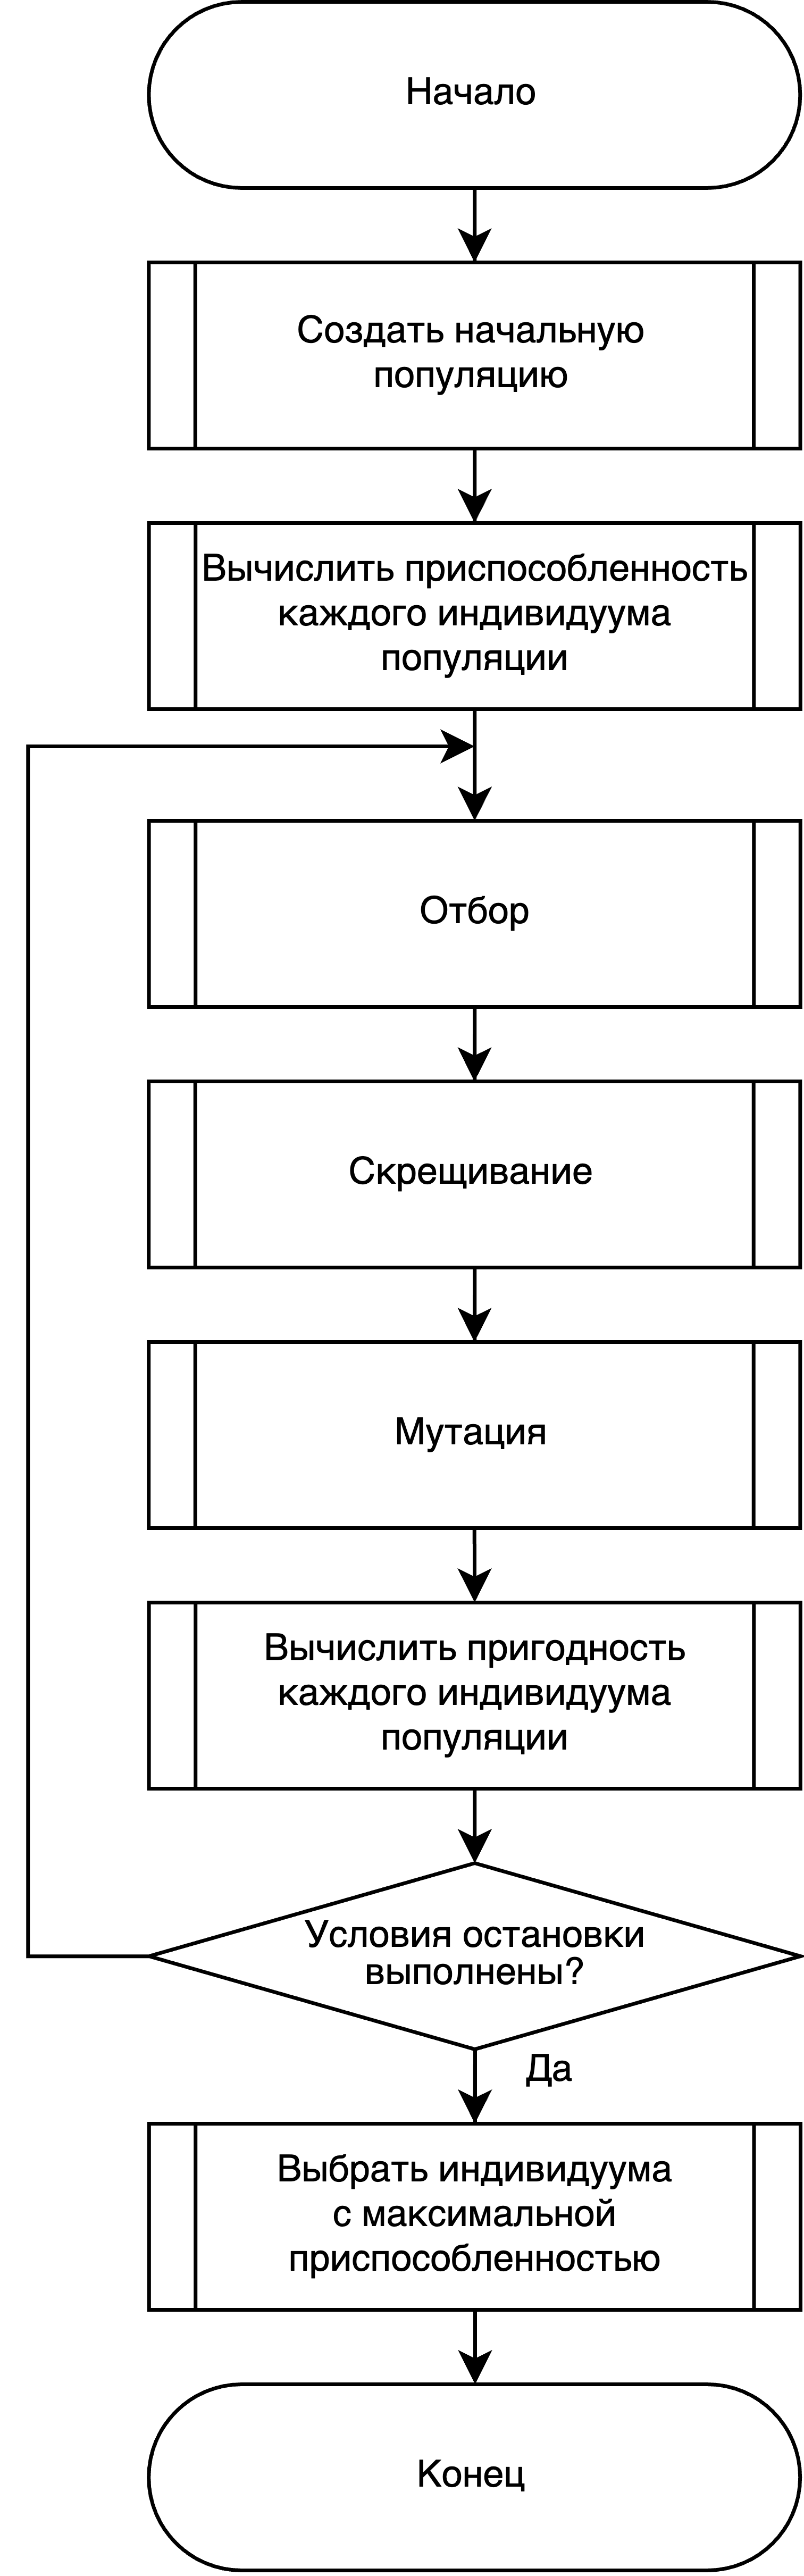
\includegraphics[height=0.95\textheight]{images/algo.png}
	\end{center}
	\caption{Основные этапы работы генетического алгоритма}
	\label{img:algo}
\end{figure}



\clearpage
